\documentclass{article}

\usepackage[margin=1in]{geometry}
\usepackage{graphicx} 
\usepackage{gensymb}
\usepackage{amsmath}
\usepackage{multicol}
\usepackage{hyperref}
\usepackage[font=small,labelfont=bf]{caption}

\begin{document}
\begin{titlepage}
    \begin{center}
        \vspace*{1cm}
            
        \Huge
        \textbf{GANs for financial time series}
            
        \vspace{0.5cm}
        \LARGE
        Using generative adversarial networks to generate financial time series
            
        \vspace{1.5cm}
            
        \textbf{Riccardo Bollati}\\
        \textbf{Elisa Carucci}\\
        \textbf{Stefan Huber}

            
        \vfill
            
        A report presented for the Project course IASP 4090\\
            
        \vspace{0.8cm}
            
        \Large
        The Chinese University of Hong Kong\\
        Hong Kong\\
        09/12/2022
            
    \end{center}
\end{titlepage}

% Elisa ------------------------------------------------------------------------------------------------------------------------------------------------

\begin{center}
    {\huge{Introduction}}
\end{center}  
\begin{multicols}{2}
    Financial time series are useful for various purposes, for example for training machine learning models or as inputs in market simulators. In these applications, a constraint is the limited availability of large amounts of data. This can have an impact on the performance of the analysis. For these reasons, models, especially deep-learning ones, tend to overfit and struggle at generalizing. By augmenting a dataset with articially generated time series, we can contribute to the solve of these issues by providing a larger amount of data with respect to what is already accessible. This can help companies and academic institutions alike to effectively improve models and use it to enhance strategy backtesting. 
    \subsection*{Characteristics of Time series}
    GANs can capture the temporal structures of financial time-series so as to generate the major stylized facts of price returns, including the linear unpredictability, the fat-tailed distribution, volatility clustering, the leverage effects, the coarse-fine volatility correlation, and the gain/loss asymmetry. 
\end{multicols}    

    \begin{center}
        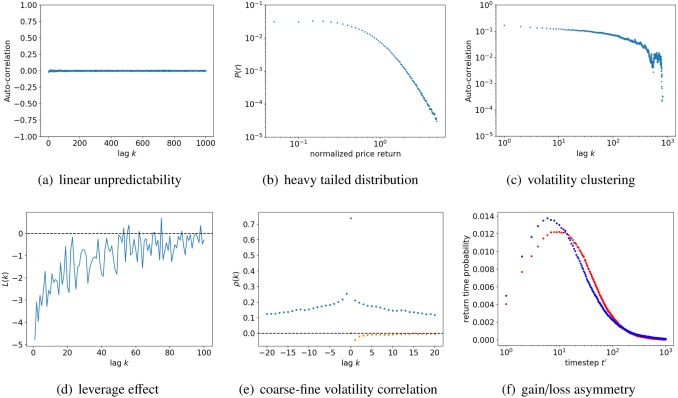
\includegraphics[scale = 0.7]{imgs/elisa/ts.jpg}
    \end{center}
    \begin{multicols}{2}

    In the studies of financial time-series, there are two major approaches, namely stochastic processes, and agent-based models, for modeling the financial time-series. However, it is difficult to recover all the major stylized facts with such explicit mathematical formulations. As an alternative approach, GANs have shown spectacular ability in the generation of data including realistic image, audio, natural language text, and financial data.\\
    
    \subsection*{General Idea}
    We began by taking a dataset of value stocks from the S\&P 500 as we assumed it would have been easier to analyze financial series with more convenient intrinsic properties such as moderate volatility. In this way it was easier to interpret the results of our model since we could identify out of range peaks very easily. The reasoning grounded on the fact that it is very hard to judge the performance of a model like this without a defined metric, which is yet to be developed. As for now, we rely on our visual interpretation.\\ \\ \\
    
    \subsection*{Scaler method}
    Since the aim of the project is to augment a dataset that can be used for further training in machine learning, we want to select the generated data that maintain the statistical properties mentioned above. For this reason we will apply a correction algorithm to correct the range of peaks of volatility. We could better observe the results thanks to the choice of our first dataset of stocks with low volatility. It was possible to capture the strange pattern of the series generated since some results did not mimic correctly the normal behavior of certain types of stocks.\\ 
    
    \subsection*{Implementation and Analysis}
    GANs were first used to give images as output so it can be hard to model different kinds of data. In our case we first tried to input prices to get back a financial series that could still preserve the statistical porperties of what we used as input. Unfortunately this was not the case as the series did not mimic the real dataset well. In fact we can see how the mean was fixed around zero. Of course, there is a mathematical explanation behind this and we will discuss this topic in subsequent chapters.\\
    
    \begin{center}
        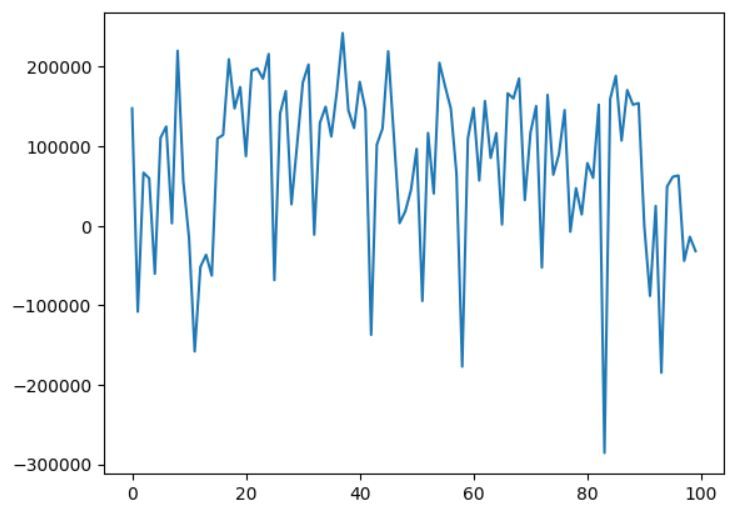
\includegraphics[scale = 0.3]{imgs/elisa/price.jpg}
    \end{center}

    Then, we decided to train the model using net returns which worked and therefore we continued our analysis with these data. As we went on with the implementation of the model, we encountered a problem in terms of randomization.\\

    \begin{center}
        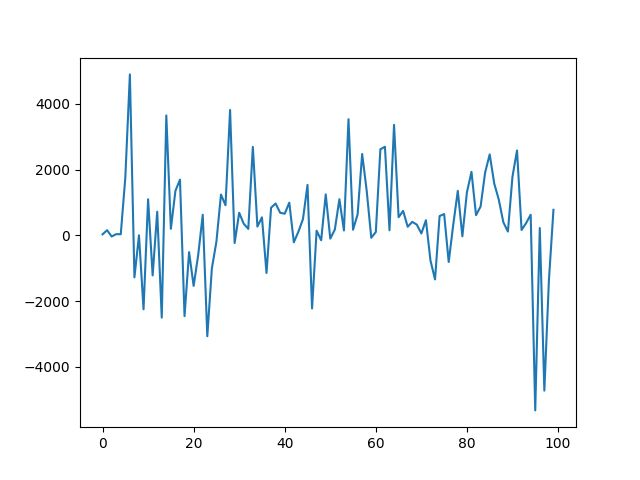
\includegraphics[scale = 0.2]{imgs/elisa/1.jpg}
        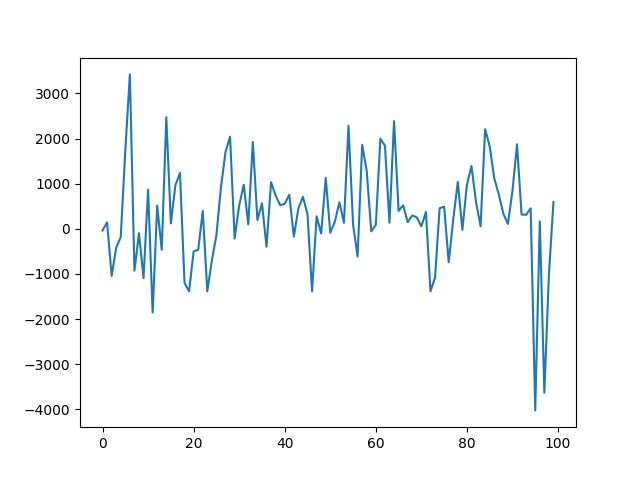
\includegraphics[scale = 0.2]{imgs/elisa/2.jpg}
        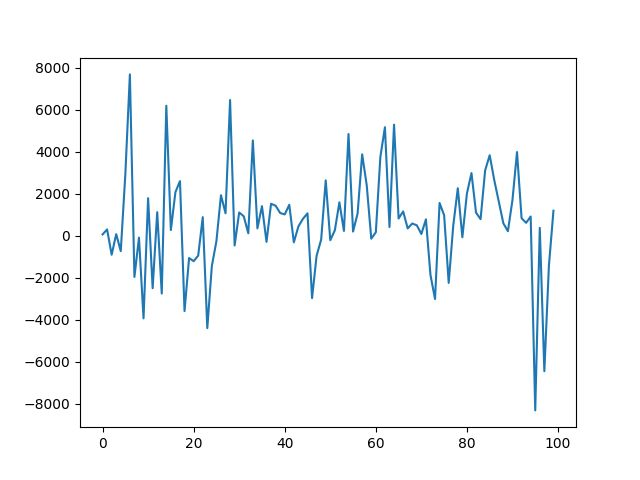
\includegraphics[scale = 0.2]{imgs/elisa/3.jpg}
        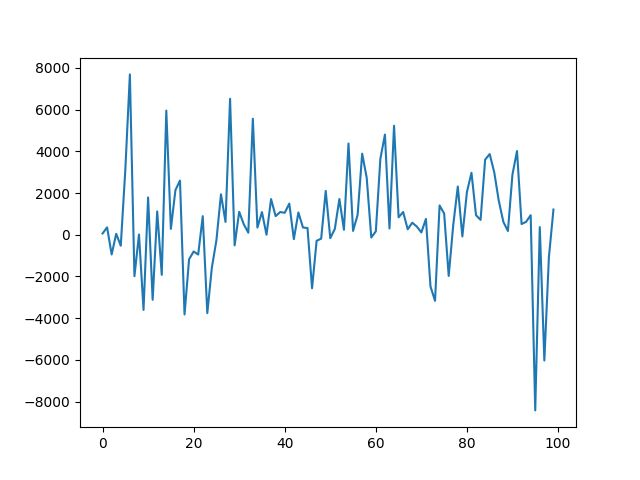
\includegraphics[scale = 0.2]{imgs/elisa/4.jpg}
    \end{center}

    In order to solve this problem we took away the spectral normalization from the generator after doing some trials also with respect to the discriminator. At the end of this process we finally got realistic results which will be shown later in the paper. It is also with these results that we applied the scalar method explained later. \\

    On the other side, we also tried to test the model on log returns with negative results.\\

    \begin{center}
        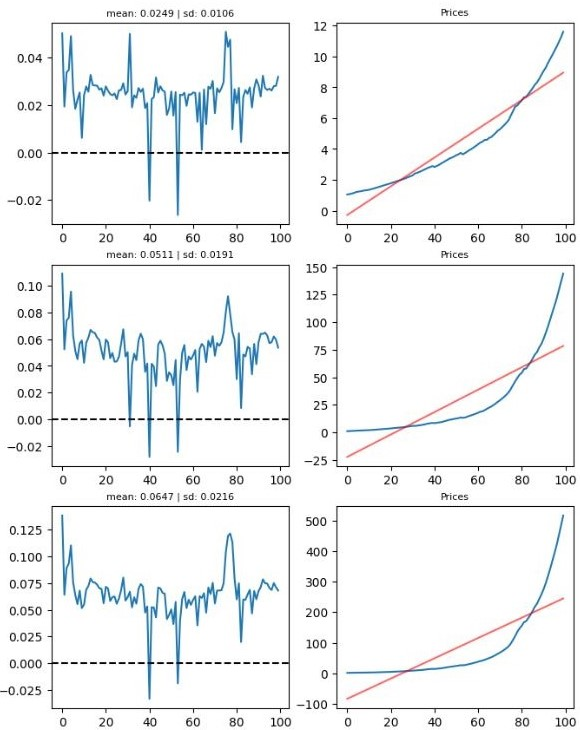
\includegraphics[scale = 0.5]{imgs/elisa/log.jpg}
    \end{center}

    The mean is not around zero as with the net returns. We will now discuss more about these results by comparing the tyoes of returns to be used in financial data analysis.\\

    \subsection*{Returns}
    Prices between assets may be difficult to compare. For example, a large company might have a higher stock price than a smaller competitor. However, the bigger company's price could be relatively stable, while the competitor's smaller price is rapidly increasing. Thus, naturally one wants to think of prices in relative terms. Let's denote the price of an asset at time t. Then the return of an asset captures these relative movements and is defined as:
    $$r_t = \frac{p_t - p_{t-1}}{p_{t-1}}$$
    In words, a return is the change in price of an asset, relative to its previous value. In practice, “returns” often means “log returns”. Log returns are defined as:
    $$z_t = \log(1+r_t)$$
    Returns are lower-bounded by -1.0. One cannot lose more than all of one's money. However, log returns have an infinite support. And since the log function suppresses big positive values while emphasizing small negative values, log returns are more symmetric than returns. This is a natural consequence of logarithms.\\
    In terms of distribution, net returns follow the normal distribution which is symmetric. The lognormal distribution (of log/geometric returns) is not. It's slightly skewed/biased. This happens because the log function is concave around 1, which means it returns "more negative" numbers for values less than 1 than the positive values it returns for numbers the same distance greater than 1. In practice this means that when simple returns average zero, log returns are negative, since negative returns have a more negative log return than "equal" positive returns. If your arithmetic mean is positive but close to zero, then it's not unusual to have a small negative log return average. 
    
    \subsection*{Statistical properties of financial time series}
    The final goal for a GAN is to preserve the statistical properties of the data used. We list the most important ones to evaluate the results below. However for now, we will limit our evaluation to a qualitative visual interpretation and the comparision of one statistical property, the mean. For future work it would be desireable to create a framework to measure performance of GANs in creating financial time series.\\
    \subsection*{Linear unpredictability}
    The first fundamental property of financial time-series is its linear unpredictability. This property is quantified by the diminishing auto-correlation function of price return. \\
     \begin{center}
        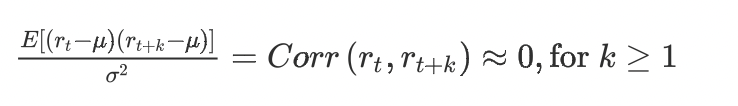
\includegraphics[scale = 0.6]{imgs/elisa/lp.jpg} 
    \end{center}
    The figure shows the decay of the auto-correlation function of the price return in daily scale. The absence of linear correlation in the price return in daily scale implies that the financial markets are efficient to a certain extent.\\
    \subsection*{Fat-tailed distribution}
    The probability distribution has a power-law decay in the tails. A heavy tailed distribution has tails that are heavier than an exponential distribution.  In other words, the tails simply look fatter. As the tails have more bulk, the probability of extreme events is higher compared to the normal. 
    \begin{center}
        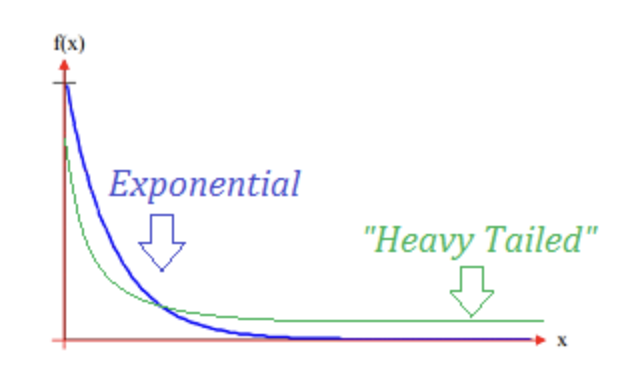
\includegraphics[scale = 0.6]{imgs/elisa/dist.jpg} 
    \end{center}
    

    \subsection*{Volatility clustering}
    While the auto-correlation of the price return is absent, there is still an important temporal structure in the financial time-series, namely volatility clustering. Qualitatively speaking, volatility clustering refers to the fact that the large/small price fluctuations tend to cluster together temporally. Quantitatively, volatility clustering is characterized with the power-law decay of the auto-correlation function of the absolute price returns. 
    \begin{center}
        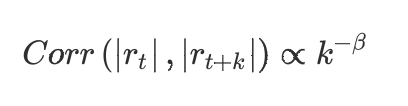
\includegraphics[scale = 0.8]{imgs/elisa/cl.jpg} 
    \end{center}

\end{multicols}

% STEFAN -------------------------------------------------------------------------------------------------------------------------------------
\begin{center}
    {\huge{GAN architecture}}
\end{center}  

\begin{multicols}{2}
    \section{Introduction}
    In order to generate the time series of a similar distribution as the original ones, we chose to use a Generative Adversarial Network (GAN). The GAN framework consists of two models, the generator and the discriminator. They learn by “playing” against each other: The generator generates new time series and tries to trick the discriminator into predicting them as real ones, while the predictor learns to distinguish them. Ideally in this process, the predictor learns the distribution of real data and the generator generates series that share exactly this distribution, such that ultimately the discriminator's best choice is to pick at random. \\
    Regarding the architecture of generator and discriminator, we draw significant inspiration from Savasta \& Politano (2020). We used a Wasserstein GAN, as this improves training stability and the loss directly correlates with the sample quality, so for more advanced performance evaluation we later can just use the loss function of the generator rather than only see whether the model can fool human eyes.
    \section{A first Generator}
    A first Generator
    The architecture is mainly a combination of linear and convolutional layers and was designed by Fernando (2019), but as Savasta \& Politano (2020) we use RMSprop as optimizer rather than adam. In contrast to them however, we completely remove spectral normalization as it caused model collapse. We use the Xavier uniform initializer to initialize the weights of the model. That way we ensure that the weights of the network are initialized in a way that is well-suited to the activation functions used in the network. This helps to improve the performance of the network by ensuring that the weights are not too small or too large, which can prevent the network from learning effectively. \\
    The generator takes a random noise vector of length 50 as input returns a time series vector of length 100. It consists of several layers, each of which applies a different transformation to the input data. The first layer is a linear transformation, which applies a matrix multiplication and a bias term to the input data. This is followed by a Leaky ReLU nonlinearity, which applies a nonlinear function element-wise to the input data. The next layer adds an extra dimension to the input data, which is necessary for the subsequent convolutional layers. \\
    Then three 1D convolutional layers follow, which apply a convolution operation to the input data. This operation is a way of extracting local spatial information from the input data. The convolution is followed by an upsampling operation, which increases the size of the data. The upsampling is followed by a dropout layer, which randomly zeroes out some of the input data. This prevents overfitting and increases robustness. Then a fourth convolutional layer follows. \\
    Finally a Leaky ReLU applies an element-wise nonlinear function to the input data and the data get squeezed down to a single dimension, and the last layer is a linear transformation, which applies a matrix multiplication and a bias term to the input data.
    \begin{center}
        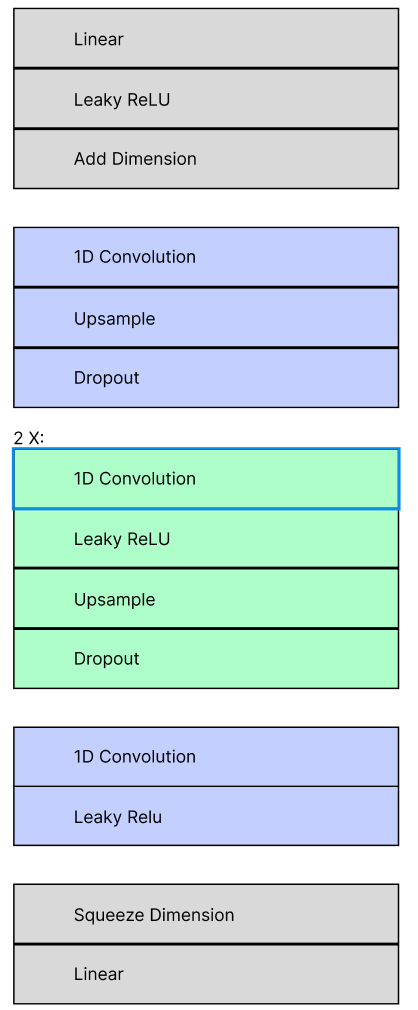
\includegraphics[scale=0.3]{imgs/stefan/generator-graphic-v1.png}
    \end{center}

    \section{The Discriminator}
    The discriminator, also called critic, takes in the generated time series or the original ones as input and returns a single number, indicating whether it predicts the input to be an original or generated time series. With respect to its architecture the critic is very similar to the generator. \\
    At first it adds an extra dimension to the input data, which is necessary for the subsequent convolutional layers. Three 1D convolutional layers follow, which apply a convolution operation to the input data to extract local spatial information from the input data. We use spectral normalization to increase training stability as Savasta \& Politano (2020) suggest. Again, the convolution is followed by a Leaky ReLU nonlinearity, which applies a nonlinear function element-wise to the input data. The convolution is also followed by a max pooling operation, which reduces the size of the data by taking the maximum value within a local neighborhood of each element. \\
    The next three layers are fully-connected (i.e., linear) layers with varying sizes, which apply a matrix multiplication and a bias term to the input data. These also have Leaky ReLU nonlinearities. The final layer produces a single output value, indicating whether the input data is real or fake.
    \begin{center}
        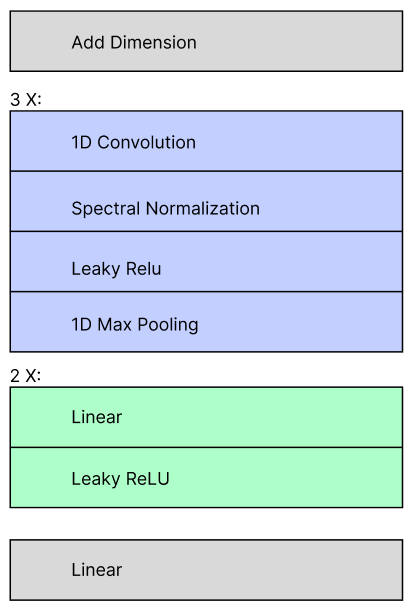
\includegraphics[scale=0.3]{imgs/stefan/discriminator-graphic-v1.png}
    \end{center}    
\end{multicols}

% RICCARDO ------------------------------------------------------------------------------------------------------------------------
\vspace{0.3cm}
\begin{center}
    {\huge{How the Scaler function works}}
\end{center}    
    \begin{multicols}{2}
    The main problem of the data generated by the model is the scale of the data itself.
    As we can see in the following picture, the series seems realistic if we just look at the trend.
    However, the magnitude of the data is totally out of scale. The algorithm below is designed to force
    the series to converge to the real data range.
    \subsection*{Introduction}
    The scaler aims at scaling the time series without affecting the trend. The idea is that when we have 
    a peak of returns in the time serie, the significance of the peak depends on its distance from the second highest peak in the serie. For exemple let's take the following series from the dataset of stock values:\\
    \begin{center}
        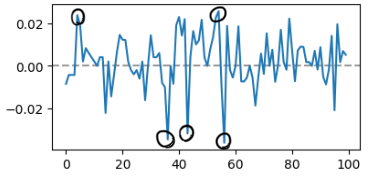
\includegraphics[scale = 0.7]{imgs/riccardo/small_peaks.png}
        \captionof{figure}{}
        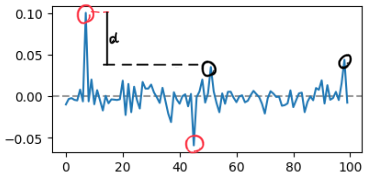
\includegraphics[scale = 0.7]{imgs/riccardo/big_peaks.png}\\
        \captionof{figure}{}
    \end{center}
    As we can see the in (\textbf{Figure 1}) the 2 highest peaks are not very far from each other. This makes the order of magnitude lower compared to the peak we can see in the (\textbf{Figure 2}). Let's analyze two different meanings a peak can refer to:
    \begin{itemize}
        \item a strong movement in price
        \item a shock, due to news or particural events.
    \end{itemize}  
    Taking into consideration the nature of the sample taken, it is very unlikely to have two big shocks in the same window. Following this logic, when the $1^{st}$ and $2^{nd}$ peaks in a series are close, we can conclude they are probably just strong movements in the price. Again, when the $1^{st}$ peak in terms of magnitude is way bigger than the $2^{nd}$, it is unlinkely to have price movements with this elevated magnitude, in very small ranges. We can note that since the usual price movement of these kind of stocks falls between a range of -0.01\% and 0.01\%, It seems reasonable to apply the scaler function to get an ultimate generated series that can be used for data analysis purposes while reflecting the true nature of the financial asset. 
    \subsection*{Scaler Logic}
    Following this reasoning, the scaler assigns the value that shocks typically have in real data, to isolated peaks in the generated series, adjusting it to a value plausible in real scenarios.
    It also assigns values typical for strong market movements to peaks very close to each other.
    \subsection*{Scaler Implementation}
    The scaler computes the quantiles of the maximum values in the distribution and for the distribution of the difference between the $1^{st}$ and 
    $2^{nd}$ peaks.\\
    Then the algorithm computes the distance between the $1^{st}$ and $2^{nd}$ peaks in the sample compared to the quantiles of the differences for real 
    data. A random value is then sampled from a uniform distribution where the lower and upper bonuds are the corresponding quantiles in the maximum distribution. 
    The same functions are applied to the negative peaks.
    \end{multicols}
    \textbf{Exemple:}
    \begin{center}
        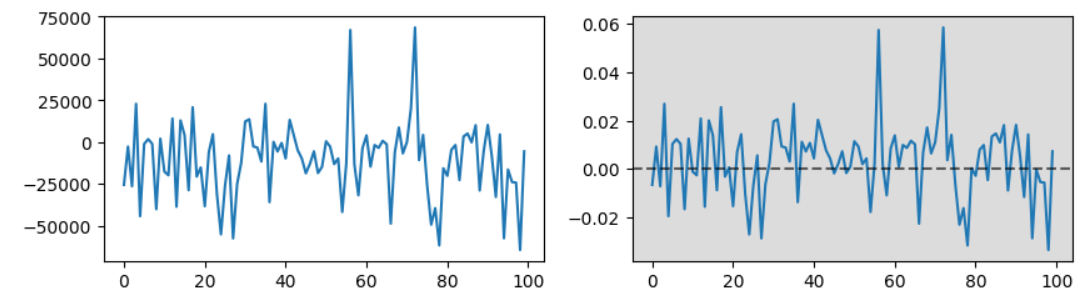
\includegraphics[scale=0.6]{imgs/riccardo/EX_03.png}
    \end{center}
    In the above exemple on the left we can see the series our model generated and on the right the series after the scaler is applied. As we can see,  
    the scaler preserves the pattern generated by our model but rescales the data such that we have realistic data we can use for other experiments and implementations.


    \vspace{0.3cm}
\begin{center}
    {\huge{Filter}}
\end{center}    
    \begin{multicols}{2}
    \section*{Problem}
    One problem we noticed in the samples our model generated after the application of the scaler is, that some are decent and realistic, but others are 
    nonsense, as is illustrated in the exemples below:
    \begin{center}
        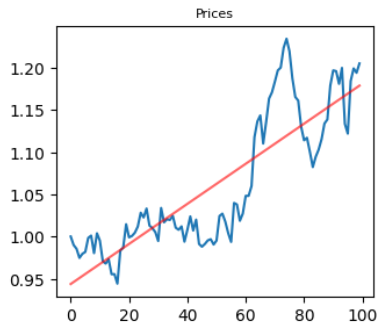
\includegraphics[scale=0.49]{imgs/riccardo/serie_comp_1.png}
        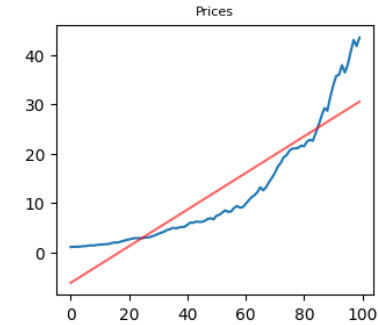
\includegraphics[scale=0.49]{imgs/riccardo/serie_comp_2.png}
    \end{center}
    As we can see, the first series is realistic but the other one is not only out of scale but shows a trendline that is very 
    atypical for fiancial time series. In order to solve this problem, we created a filter that selects from the samples generated the realistic series without modifyng the model output, that way we end up with a realistic series dataset.
    \section*{How It works}
    To select the realistic series we came up with several metrics, the value of which can be tuned in the filter parameters:
    \paragraph*{Distance between residuals.}
    We noticed that if we apply a linear regression to a series, the distance between consecutive residuals is significantly smaller when the series shows an unrelistic behavior.
    In contrast, for more realistic series the discance between consecutive points residuals is bigger.
    \begin{center}
        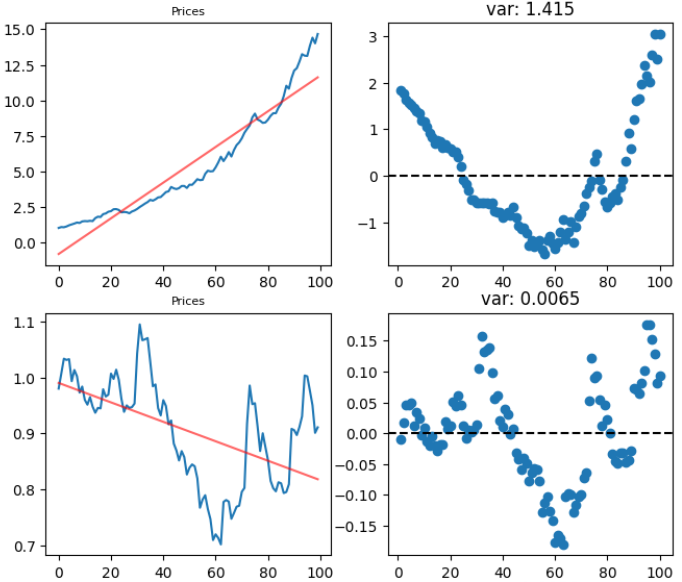
\includegraphics[scale=0.6]{imgs/riccardo/2_res.png}
    \end{center}
    We scaled the price of the generated series to the range form 0 to 1 to in order to make it comparable. Then we applied linear regression and computed the sum of the distance between consecutive residuals. 
    Then the filter just selects the series with a sum of consecutive residuals above a given threshold.\\
    \textbf{DfGenerator parameter}:  \textbf{variance\_th}.
    \paragraph*{Maximum range of oscillation}
    We decided to introduce a parameter in the filter to chose the maximum range of oscillation between the first point an the last one in percentage. This is because we think it could be useful to have the freedom to decide the type of series we want 
    to generate to expand our dataset. Potentially we would want to expand our dataset with very volatile series, in which case we can chose to use a high maximum range of osscilation. Alternatively, our need could be to expand our dataset with more stable series, for example in order to decrease 
    the volatility of the predictions made by a model. In that case we can tune the parameter chosing a lower maximum range.\\
    \textbf{DfGenerator parameter}:  \textbf{max\_range}.

    \end{multicols}
    \newpage
    \begin{center}
        {\huge{Final Results}}
    \end{center} 
    The final result of the project is a program capable of generating seemingly realistic financial series such the following:
    \begin{center}
        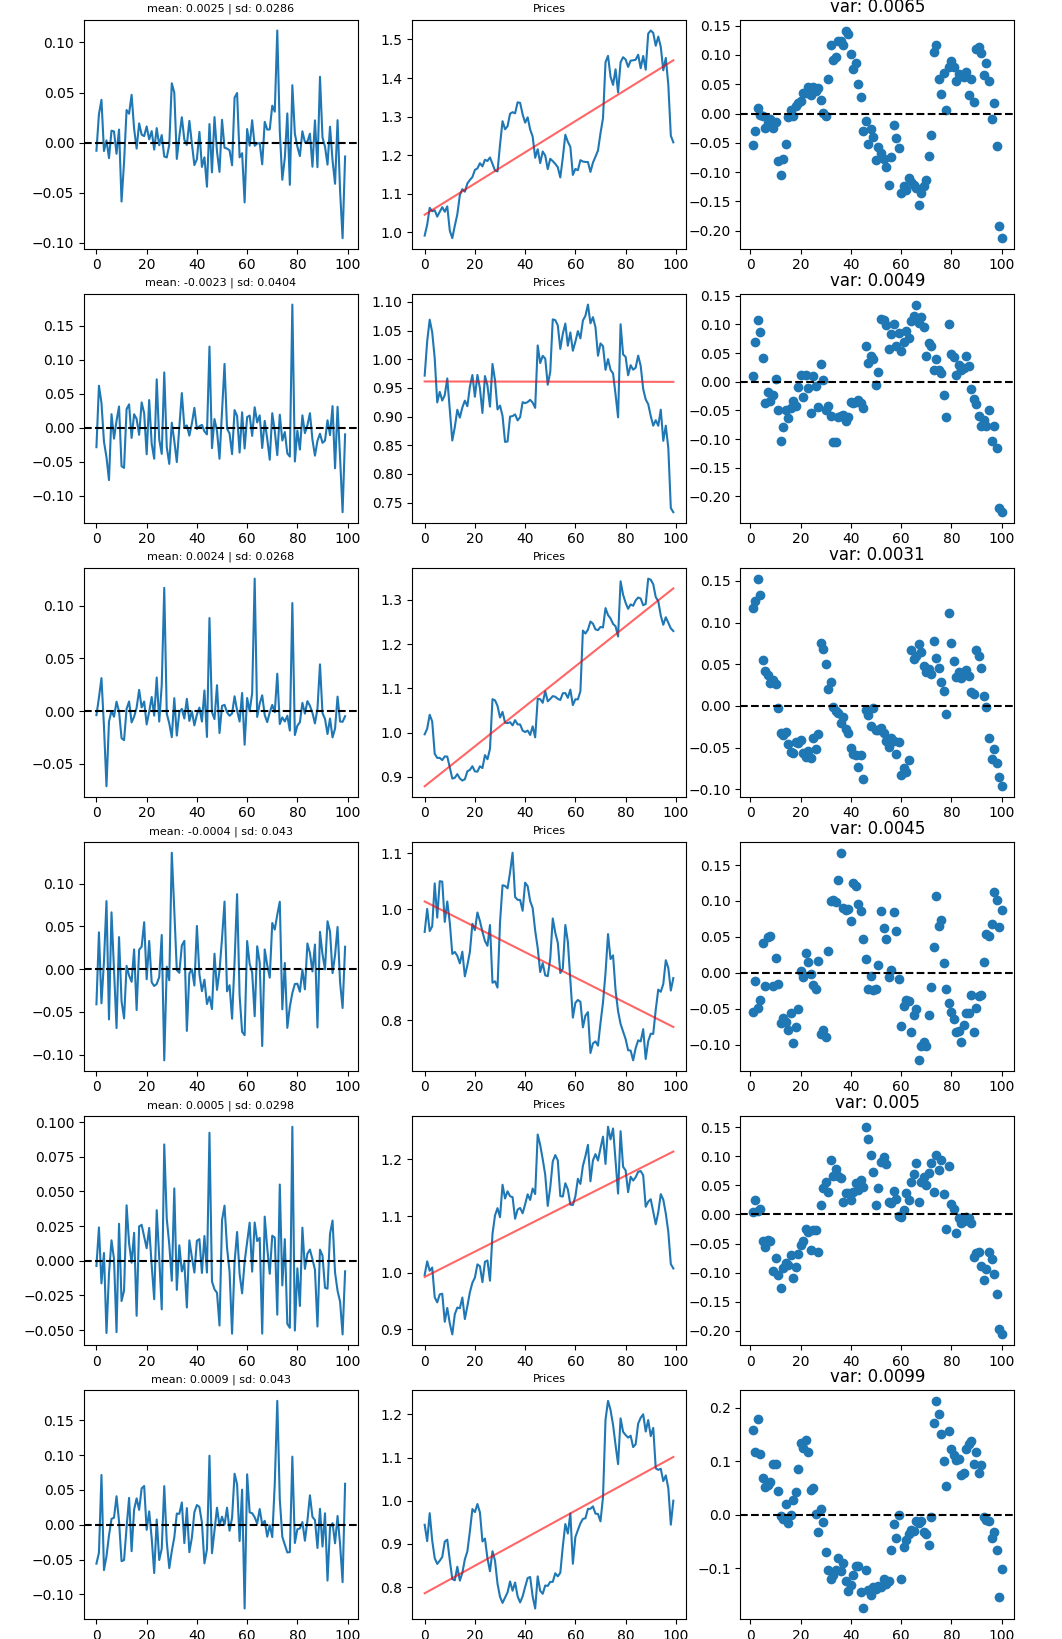
\includegraphics[scale=0.5]{imgs/riccardo/results_reduced.png}
    \end{center}
    \newpage
    The generated series are visually similar to the original series. In the graph, the generated series have a grey background to distinguish them from the original ones:
    \begin{center}
        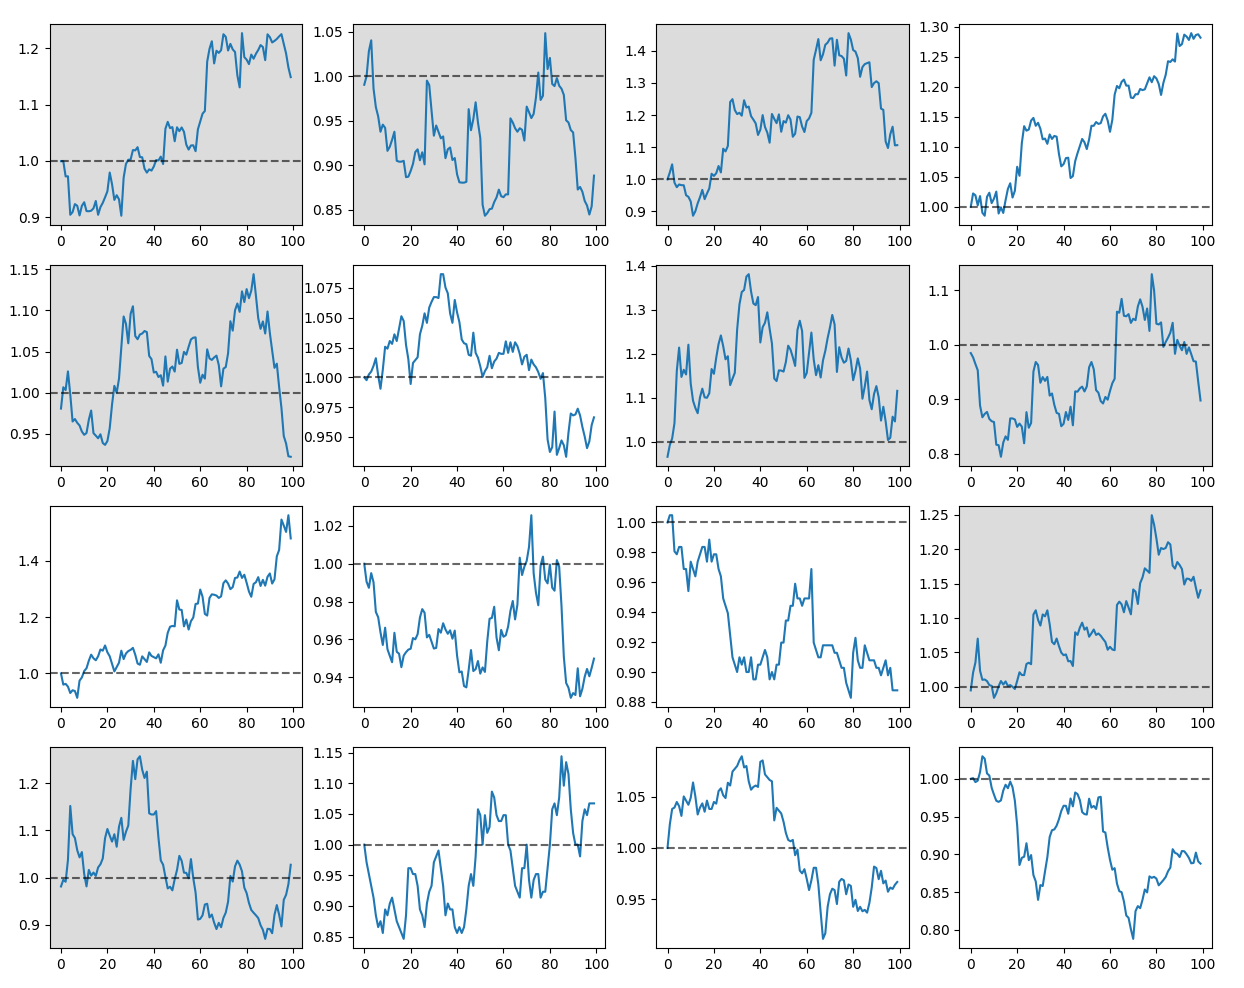
\includegraphics[scale=0.5]{imgs/riccardo/series_comparison_README.png}
    \end{center}
    One of the main characteristics of returns of financial products is that the mean is almost equal to 0.
    We generated a dataset of 10 000 samples, which yields computed mean of 0.00026567.
    The program takes approximatly 20 mintutes to generate a 10 000 samples dataset on a single CPU Intel Core I7. The means of the generated samples are distributed as follows:
    \begin{center}
        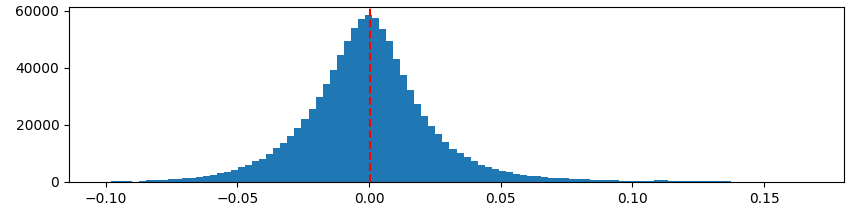
\includegraphics[scale=0.75]{imgs/riccardo/generated.png}
    \end{center}
    
    \newpage
    \begin{center}
        {\huge{Future Work}}
    \end{center} 
    This is a list of future work improving upon our project:
    \begin{enumerate}
        \item Develop a robust testing framework to evaluate generated time series datasets
        \item Test and compare a wider set of architectures
        \item Implement a tensorboard interface to check model performance in realtime during the training
        \item Inlcude the rescaler in the model architecture of the generator such that the quantiles can be optimized during the training or get completely rid of the need for it
        \item Test the models performance on different types of datasets (e.g. specific sectors stocks) to see how this affects the results
        \item study the statistical properties of the series generated
        \item Expand a datataset and see how this affects the performance of a prediction model
    \end{enumerate}

    % \cite{Mindermann_2022}
    
    \begin{thebibliography}{9}
        \bibitem{Mindermann_2022}
        Mindermann, S., et al. (2022) \emph{Prioritized Training on Points that are learnable, Worth Learning, and Not Yet Learnt.}, \href{https://doi.org/10.48550/arXiv.2206.07137}{arXiv.2206.07.137}.
        
        \bibitem{}
        \end{thebibliography}

\end{document}

